\documentclass[11pt]{article}

%%%%%%%% CREATE DOCUMENT STRUCTURE %%%%%%%%
%% Language and font encodings
\usepackage[spanish]{babel}
\usepackage[utf8x]{inputenc}
\usepackage[T1]{fontenc}
%\usepackage{subfig}

%% Sets page size and margins
\usepackage[a4paper,top=3cm,bottom=2cm,left=2cm,right=2cm,marginparwidth=1.75cm]{geometry}

%% Useful packages
\usepackage{amsmath}
\usepackage{graphicx}
\usepackage[colorinlistoftodos]{todonotes}
\usepackage[colorlinks=true, allcolors=blue]{hyperref}
\usepackage{caption}
\usepackage{subcaption}
\usepackage{sectsty}
\usepackage{apacite}
\usepackage{float}
\usepackage{titling} 
\usepackage{blindtext}
\usepackage[square,sort,comma,numbers]{natbib}
\usepackage[colorinlistoftodos]{todonotes}
\usepackage{xcolor}
\definecolor{darkgreen}{rgb}{0.0, 0.4, 0.0}
\usepackage{listings}
\usepackage{color}
\usepackage{fancyhdr}

\pagestyle{fancy}
\fancyhf{}
\fancyhead[LE,RO]{IPS 2022}
\fancyhead[RE,LO]{Instalación y Reemplazo de Componentes Internos}
\fancyfoot[CE,CO]{\nouppercase\leftmark}
\fancyfoot[LE,RO]{\thepage}

\renewcommand{\headrulewidth}{2pt}
\renewcommand{\footrulewidth}{1pt}
\definecolor{dkgreen}{rgb}{0,0.6,0}
\definecolor{gray}{rgb}{0.5,0.5,0.5}
\definecolor{mauve}{rgb}{0.58,0,0.82}

\usepackage{caption}
\usepackage[newfloat]{minted}
\captionsetup[listing]{position=top}


\newcommand{\subsubsubsection}[1]{\paragraph{#1}\mbox{}\\}
\setcounter{secnumdepth}{4}
\setcounter{tocdepth}{4}
\usepackage{xpatch}
\usepackage{booktabs}

\makeatletter
\AtBeginEnvironment{minted}{\dontdofcolorbox}
\def\dontdofcolorbox{\renewcommand\fcolorbox[4][]{##4}}
\xpatchcmd{\inputminted}{\minted@fvset}{\minted@fvset\dontdofcolorbox}{}{}
\xpatchcmd{\mintinline}{\minted@fvset}{\minted@fvset\dontdofcolorbox}{}{}
\makeatother

%%%%%%%% DOCUMENT %%%%%%%%
\begin{document}
\begin{large}
%%%% Title Page
\begin{titlepage}

\newcommand{\HRule}{\rule{\linewidth}{0.5mm}} 							% horizontal line and its thickness
\noindent\begin{minipage}{0.3\textwidth}% adapt widths of minipages to your needs

\includegraphics[scale=0.5]{img/Titulo/unr.png}
\end{minipage}%
\hfill%
\begin{minipage}{0.6\textwidth}\raggedleft

\includegraphics[scale=0.25]{img/Titulo/Logo IPS upscaled.png}
\end{minipage}

\vspace{5mm}

\hline

\vspace{7.5mm}

\center 
 
% University
\textsc{\LARGE Instituto Politécnico Superior "General San Martín"}\\[1cm]

% Document info
\textsc{\Large Instalación y Reemplazo de Componentes Internos}\\[0.2cm]				
\vspace{7.5mm}

\HRule \\[0.8cm]
{ \huge \bfseries Práctica 2 MIPS (Cuestiones)}\\[0.7cm]								% Assignment
\HRule \\[2cm]
\large
\emph{Autor:}\\
Juan Ignacio Bertoni\\[1.5cm]	
\emph{Curso:}\\
6to Año Informática\\[1.5cm]	
\emph{Docente:}\\
Alejandro Rodriguez Costello\\[1.5cm]	

% Author info
{\large \today}\\[5cm]
\vfill 
\end{titlepage}



\vfill

\begin{flushleft}

\section*{Evaluación de expresiones}
\subsection*{Cuestión 1.1}

El valor cargado en la posición de memoria \textbf{res} es \texttt{1}, pues resulta \texttt{t0<t1}. 

\subsection*{Cuestión 1.2}
El valor cargado en la posición de memoria \textbf{res} es \texttt{0}, pues no resulta \texttt{t0<t1}. 

\subsection*{Cuestión 1.3}
Se ha evaluado si t0 era menor a t1. Al no serlo, el registro \$t2 fue puesto a 0 (falso).

\subsection*{Cuestión 1.4}
Del código del apartado anterior, lo que habría que hacer es reemplazar la línea en la que se llama a la instrucción \texttt{slt} y en cambio llamar a \texttt{seq} (set if equal).

\begin{listing}[h]
\begin{minted}[linenos,frame=single]{nasm}
seq $t2,$t0, $t1 # poner a 1 $t2 si t0==t1
\end{minted}
\end{listing}

\subsection*{Cuestión 1.5}
Utilizando la instrucción \texttt{sge}, el código se vería de la siguiente manera:
\begin{listing}[h]
\begin{minted}[linenos,frame=single]{nasm}
.data
dato1: .word 10
dato2: .word 10
res: .space 1
.text
main: lw $t0,dato1($0) # cargar dato1 en t0
lw $t1,dato2($0) # cargar dato2 en t1
sle $t3,$t0, $t1 # poner a 1 $t2 si t0<=t1
sge $t4,$t0, $t1 # poner a 1 $t2 si t0>=t1
and $t2, $t3, $t4 # poner a 1 $t2 si t0==t1

sb $t2,res($0) # almacenar $t2 en res
\end{minted}
\end{listing}

Al hacer un \texttt{and} entre ambos registros (set if less or equal y set if greater or equal), en definitiva estoy preguntando si ambos registros son iguales o no.


\subsection*{Cuestión 1.6}

El valor cargado en \texttt{res} en este caso es \texttt{1}, pues ocurre que \texttt{t0$<$t1} (\texttt{30$<$40}).


\subsection*{Cuestión 1.7}
El valor cargado en \texttt{res} en este caso es \texttt{0}, pues no ocurre que \texttt{t0$<$t1} (\texttt{50$>$20}).

\subsection*{Cuestión 1.8}
El valor cargado en \texttt{res} en este caso es \texttt{0}, pues no ocurre que \texttt{t0$<$t1} (\texttt{20==20}).

\subsection*{Cuestión 1.9}
En el programa entero podemos ver que se evalua la expression \texttt{t0$<=$t1}, pues primero se pregunta si t0 es menor o igual que t1 a través de la intrucción \texttt{slt}. Luego, si dicha condición no se cumplió podría implicar que t0 y t1 son iguales. En ese caso, se utiliza un cambio de rama condicional \texttt{branch if not equal} que se saltea la intrucción \texttt{ori}. La instrucción \texttt{ori (or immediate)} se encarga de convertir el valor de \$t2 a 1, así siendo la resolución 1 si se cumplió \texttt{t0 == t1} o \textbf{t0$<$t1}.

\subsection*{Cuestión 1.10}
Una solución más simple al problema hubiera sido a través del uso de la pseudo-instrucción \texttt{sle (set if less or equal).}

\begin{listing}[h]
\begin{minted}[linenos,frame=single]{nasm}
.data
dato1: .word 30
dato2: .word 40
res: .space 1
.text
main: lw $t0,dato1($0) # cargar dato1 en t0
lw $t1, dato2($0) # cargar dato2 en t1
sle $t2, $t0, $t1 # poner a 1 $t2 si t0$<=$t1
sb $t2,res($0) # almacenar $t2 en res
\end{minted}
\end{listing}

\subsection*{Cuestión 1.11}
La solución sin utilizar pseudoinstrucciones sería con el uso de ramas condicionales:

\begin{listing}[h]
\begin{minted}[linenos,frame=single]{nasm}
.data
dato1: .word 30
dato2: .word 40
res: .space 1
.text
main: lw $t0,dato1($0) # cargar dato1 en t0
lw $t1, dato2($0) # cargar dato2 en t1
sgt $t2, $t0, $t1 # poner a 1 $t2 si t0>t1
bne $t0,$t1,fineval # si t0<>t1 salta a fineval
ori $t2,$0,1 # poner a 1 t3 si t0=t1
fineval: sb $t2,res($0) # almacenar $t2 en res
\end{minted}
\end{listing}

\subsection*{Cuestión 1.12}
Para lograr el mismo resultado, pero utilizando pseudo-instrucciones haremos uso del \texttt{sge (set if greater or equal)}.

\begin{listing}[h]
\begin{minted}[linenos,frame=single]{nasm}
.data
dato1: .word 30
dato2: .word 40
res: .space 1
.text
main: lw $t0,dato1($0) # cargar dato1 en t0
lw $t1, dato2($0) # cargar dato2 en t1
sge $t2, $t0, $t1 # poner a 1 $t2 si t0>=t1
sb $t2,res($0) # almacenar $t2 en res
\end{minted}
\end{listing}

\section*{Evaluación de condiciones compuestas por operadores lógicos
``and'' y ``or''.}


%% hacer diagrama de flujo
\subsection*{Cuestión 1.13}
Lo que ocurre en el programa es lo siguiente: primeramente, inicializa el valor de los registros \$t0 y \$t1 a \texttt{0} a través de un \texttt{and} entre el registro mismo y \texttt{\$0}. Luego, pregunta si el primer valor almacenado en el registro es 0 y, en ese caso, salta condicionalmente a la branch de etiqueta \texttt{igual}, saltándose así la instrucción \texttt{ori}, la cual se encargaba de cargarle el valor \texttt{1} al registro \texttt{\$t0}. Luego, ocurre la misma analogía con el valor almacenado en \texttt{\$t9} y el valor que almacena \texttt{\$t1} (0 si \texttt{\$t9} almacena 0 y 1 en caso contrario). Al final de la evaluación de estos valores, se realiza una comparación \texttt{and} entre ambos valores. En este caso, como ninguno de los dos valores cargados en \texttt{\$t8} y \texttt{\$t9} son 0, entonces el valor guardado en \texttt{res} es 1.



\subsection*{Cuestión 1.14}
En este caso a \texttt{res} se le carga el valor 0, pues uno de los valores entre \texttt{\$t8} y \texttt{\$t9} es 0 (en este caso, el valor de \texttt{\$t8}).




\subsection*{Cuestión 1.15}
En este caso a \texttt{res} se le carga el valor 0, pues uno de los valores entre \texttt{\$t8} y \texttt{\$t9} es 0 (en este caso, el valor de \texttt{\$t9}).

\subsection*{Cuestión 1.16}
En este caso a \texttt{res} se le carga el valor 0, pues uno de los valores entre \texttt{\$t8} y \texttt{\$t9} es 0 (en este caso, ambos valores almacenan \texttt{0}).


\subsection*{Cuestión 1.17}
La comparación evaluada entre dato1 y dato2 en definitiva sería: \texttt{((dato1 != 0) \&\& (dato2 != 0))}

\subsection*{Cuestión 1.18}
Para lograr \texttt{((dato1 $<>$ 0) and (dato1 $<>$ dato2))} lo único que deberíamos hacer sería cambiar la condición de cambio de la segunda branch, en lugar de saltar si \texttt{dato2==0}, que salte si \texttt{dato2==dato1}:

\begin{listing}[h]
\begin{minted}[linenos,frame=single]{nasm}

.data
dato1: .word 40
dato2: .word -50
res .space 1
.text
main: lw $t8,dato1($0)
lw $t9,dato2($0)
and $t0,$t0,$0
and $t1,$t1,$0
beq $t8,$0,igual
ori $t0,$0,1
igual: beq $t9,$t8,fineval
ori $t1,$0,1
fineval: and $t0,$t0,$t1
sb $t0,res($0)

\end{minted}
\end{listing}

\subsection*{Cuestión 1.19}
Lo que ocurre en el programa es lo siguiente: primeramente, inicializa el valor de los registros \$t0 y \$t1 a \texttt{0} a través de un \texttt{and} entre el registro mismo y \texttt{\$0}. Luego, pregunta si el el registro \$t8 NO es igual a 0, caso en el cual saltaría de rama condicionalmente hacia \texttt{igual}, salteándose así la asignación del valor \texttt{1} al registro \texttt{\$t0}. Luego se pregunta si el valor almacenado en \texttt{\$t9} es menor al de \texttt{\$t8}, con lo cual el valor de \texttt{\$t0} se convertiría en \texttt{1}. Finalmente, se lleva a cabo una comparación \texttt{and} entre los valores almacenados en \texttt{\$t0} y \texttt{\$t1}. En este caso, con los valores \texttt{30} en \texttt{\$t8} y \texttt{-50} en \texttt{\$t9} ocurre que \texttt{30 != 0} y \texttt{-50 $<$ 30}, y su \texttt{and} es \texttt{0}, por lo cual el valor almacenado en la etiqueta \texttt{res} es \texttt{0}.

\subsection*{Cuestión 1.20}
En este caso, \texttt{res} almacena el valor \texttt{0}, pues ninguna de las condiciones se cumplen \texttt{(10 != 0)} y \texttt{(20 > 10)}. 

\subsection*{Cuestión 1.21}
En este caso, \texttt{res} almacena el valor \texttt{1}, pues \texttt{(0 == 0)} y \texttt{(-20 $<$ 0)}. 

\subsection*{Cuestión 1.22}
La comparación compuesta que se ha evaluado es : \texttt{((dato1 == 0) \&\& (dato2 $<$ dato1))}

\subsection*{Cuestión 1.23}
El código modificado para que se cumpla ((dato1 $<>$dato2 ) and (dato1 $<=$ dato2)) sería:

\newpage

\begin{listing}[h]
\begin{minted}[linenos,frame=single]{nasm}
main: lw $t8,dato1($0)
lw $t9,dato2($0)
and $t2,$t2,$0
and $t1,$t1,$0
and $t0,$t0,$0
beq $t8,$t9,igual
ori $t0,$0,1
igual: slt $t1,$t8,$t9
bne $t8,$t9,fineval
ori $t2,$0,1
fineval: or $t1, $t1, $t2  
         and $t0,$t0,$t1
sb $t0,res($0)

\end{minted}
\end{listing}

\subsection*{Cuestión 1.24}
El código modificado para que se cumpla ((dato1 $<>$dato2 ) and (dato1 $<=$ dato2)) usando \texttt{sle} sería:

\begin{listing}[h]
\begin{minted}[linenos,frame=single]{nasm}
main: lw $t8,dato1($0)
lw $t9,dato2($0)
and $t1,$t1,$0
and $t0,$t0,$0
beq $t8,$t9,igual
ori $t0,$0,1
igual: sle $t1,$t8,$t9
fineval: and $t0,$t0,$t1
sb $t0,res($0)

\end{minted}
\end{listing}


\subsection*{Cuestión 1.25}
Lo que ocurre en el programa es lo siguiente: primeramente, inicializa el valor de los registros \$t0 y \$t1 a \texttt{0} a través de un \texttt{and} entre el registro mismo y \texttt{\$0}. Luego, se pregunta si el valor almacenado en \$t8 es menor al valor en \texttt{\$t9} y, de ser así, se pone a \texttt{1} el valor de \texttt{\$t0}. Luego, se realiza un salto de rama condicional en caso de que \texttt{\$t9} tenga almacenado un 0, caso en el cual se saltaría la asignación de \texttt{\$t1} a 1 a través de la instrucción \texttt{ori}. Finalmente, con dichos valores se lleva a cabo una instrucción \texttt{or} entre los valores en \texttt{\$t0} y \texttt{\$t1}. En este caso, como \texttt{30 > -20} y \texttt{-20 != 0} entonces el valor almacenado en \texttt{res} es \texttt{0}.



\subsection*{Cuestión 1.26}
En este caso, \texttt{res} almacena el valor \texttt{1}, pues \texttt{(10 != 0)} pero \texttt{(-20 $<$ 10)}. 



\subsection*{Cuestión 1.27}
En este caso, \texttt{res} almacena el valor \texttt{1}, pues \texttt{(10 $>$ 0)} pero \texttt{(0 == 0)}. 


\subsection*{Cuestión 1.28}
En este caso, \texttt{res} almacena el valor \texttt{0}, pues \texttt{(20 $>$ 10)} y \texttt{(10 != 0)}. 


\subsection*{Cuestión 1.29}
La comparación compuesta que se ha evaluado es : \texttt{((dato1 < dato2) || (dato2 == 0))}

\subsection*{Cuestión 1.30}
El código modificado para que se cumpla ((dato1 <= dato2) or (dato1 <= 0)) sería:
\begin{listing}[h]
\begin{minted}[linenos,frame=single]{nasm}
main: lw $t8,dato1($0)
lw $t9,dato2($0)
and $t0,$t0,$0
and $t1,$t1,$0
and $t2,$t2,$0
and $t3,$t3,$0
slt $t0,$t8,$t9
bne $t8,$t9,fineval
ori $t1,$0,1
fineval: or $t0,$t0,$t1
slt $t2, $t8, $0
bne $t8, $0, notzero
ori $t3, $0, 1
notzero: or $t2, $t2, $t3 
         or $t0, $t0, $t2
sb $t0,res($0)

\end{minted}
\end{listing}

\subsection*{Cuestión 1.31}
El código modificado para que se cumpla ((dato1 <= dato2) or (dato1 <= 0)) usando \texttt{sle} sería:

\begin{listing}[h]
\begin{minted}[linenos,frame=single]{nasm}
main: lw $t8,dato1($0)
lw $t9,dato2($0)
and $t0,$t0,$0
and $t1,$t1,$0
sle $t0,$t8,$t9
bgt $t9,$0,fineval
ori $t1,$0,1
fineval: or $t0,$t0,$t1
sb $t0,res($0)

\end{minted}
\end{listing}

\section*{Control de flujo condicional}

\subsection*{Cuestión 2.1} 
La instrucción que se encarga de evaluar la expresión (si los registros se dividen o no) es la pseudoinstrucción de salto de rama condicional \texttt{beq} (branch if equal), al cual saltará hacia la etiqueta especificada en caso de que la condición se cumpla. La condición de más alto nivel, que se suele utilizar en el pseudocódigo es la sentencia \texttt{if}, que cumple la misma funcionalidad, pero en lugar de saltar si una condición se cumple, se podría decir que se ``entra'' a un bloque determinado sólo si dicha condición se cumple.



\subsection*{Cuestión 2.2}
El conjunto de instrucciones que implementan la estructura condicional \textit{if-then} son:

\begin{itemize}
    \item En el caso del \texttt{if}, hablamos del salto condicional de rama; \texttt{beq registro1 registro2 \textbf{terminaif}}.
    \item Luego, nuestro \texttt{then} se encontraría justo después de la instrucción de salto condicional, pero antes de la etiqueta especificada a la cual saltar (\textbf{terminaif}), como lo muestra el ejemplo dado.
\end{itemize}


\subsection*{Cuestión 2.3}
El valor cargado en \texttt{res} en este caso es \texttt{71}, pues es el resultado de hacer (\texttt{$40+30+\lfloor40/30\rfloor$}).


%% hacer diagrama de flujo  
\subsection*{Cuestión 2.4}
En el caso que dato2 fuera 0, curiosamente no dio ningún error a simple vista, sino que el valor almacenado en \texttt{res} simplemente es 40, como si el cálculo hubiera sido \texttt{$40+0+0$}.


\subsection*{Cuestión 2.5}
El siguiente código traducido desde el pseudocódigo sería:
\begin{listing}[h]
\begin{minted}[linenos,frame=single]{nasm}
.data
dato1: .word 40
dato2: .word 30
res: .space 1
.text
main: 
lw $t0,dato1($0) # cargar dato1 en t0
lw $t1,dato2($0) # cargar dato2 en t1
and $t2,$t2,$0
and $t3,$t3,$0

ble $t1,$0, skip
div $t0, $t1
mflo $t2

skip: add $t3, $t0, $t1
        add $t2, $t2, $t3

sb $t2,res($0) # almacenar $t2 en res

\end{minted}
\end{listing}


\subsection*{Cuestión 2.6}
El pseudocódigo correspondiente al ejemplo sería:

\begin{listing}[h]
\begin{minted}[linenos,frame=single]{nasm}

VARIABLES
ENTERO: dato1=40; dato2=30; res;
INICIO
Si (dato2 != 0):
    Si (dato1 != 0):
        res = dato1/dato2

res=res+dato1+dato2;
FIN

\end{minted}
\end{listing}


\subsection*{Cuestión 2.7}
Las instrucciones que evalúan la condición y controlan el flujo del programa son las dos instrucciones \texttt{beq}, ambas verificando que ni el divisor (dato1) ni el dividendo (dato2) sean 0, y en dicho caso los divide. Esto representado en pseudocódigo se vería como un par de sentencias \texttt{if} anidadas o, como el nombre en español ``\texttt{si}''.


%% diagrama de flujo
\subsection*{Cuestión 2.8}
La instrucción destinada a servir como condición \texttt{if} se trata del salto condicional por rama \texttt{beq}, donde dicha condición es la condición de salida del flujo (si quiero verificar si dos numeros son iguales, entonces la condición de salida sería verificar que no fueran iguales). Por otra parte, lo que implica el no cumplimiento del salto condicional debe ir antes de la etiqueta que simboliza el cumplimiento del salto pero después de la instrucción \texttt{beq}.

\subsection*{Cuestión 2.9}
El valor almacenado en \texttt{res} nuevamente es 71, pues se realizó la misma cuenta que en el código anterior, ya que ni \texttt{40} ni \texttt{30} son iguales a \texttt{0}.

\subsection*{Cuestión 2.10}
En caso de que \texttt{dato1=0} en res se almacenará \texttt{30}. Por otra parte, si \texttt{dato2=0} en res se almacenará \texttt{40}.


\subsection*{Cuestión 2.11}
El siguiente código traducido desde el pseudocódigo sería:
\begin{listing}[h]
\begin{minted}[linenos,frame=single]{nasm}
.data
dato1: .word 40
dato2: .word 30
res: .space 1


.text
main: 
lw $t0,dato1($0) # cargar dato1 en t0
lw $t1,dato2($0) # cargar dato2 en t1
and $t2,$t2,$0
and $t3,$t3,$0

ble $t0,$0, skip
blt $t1, $0, skip
div $t0, $t1
mflo $t2

skip: add $t3, $t0, $t1
      add $t2, $t2, $t3

sb $t2,res($0) # almacenar $t2 en res

\end{minted}
\end{listing}

\newpage

\section*{Estructura de control \textit{if-then-else} con condición simple}

\subsection*{Cuestión 2.12}
El pseudocódigo correspondiente al ejemplo sería:

\begin{listing}[h]
\begin{minted}[linenos,frame=single]{nasm}

VARIABLES
ENTERO: dato1=30; dato2=40; res;
INICIO
Si (dato1 >= dato2):
    res = dato2
Sino:
    res = dato1
FIN
\end{minted}
\end{listing}

\subsection*{Cuestión 2.13}
En este caso a \texttt{res} se le carga el valor \texttt{30}, pues se trata del valor más pequeño entre él y \texttt{40}. Si \texttt{dato1=35}, entonces res almacena el valor \texttt{35}, pues el mismo sigue siendo menor a \texttt{40}.

\subsection*{Cuestión 2.14}
Podemos ver que llama a la función \texttt{slt} (set if less than), el cual almacena en el registro \$1 (at) el resultado de comparar \texttt{\$8$<$\$9} (dos registros temporales que guardan los valores que realmente estamos comparando). Luego se compara dicho valor con el registro constante \$0, y si eso ocurre entonces saltará hacia la etiqueta 4 (esta usualmente es una dirección expresada en hexadecimal, pero yo configuré el emulador para que mostrara los valores decimales). Así, da el mismo efecto saltar si no ocurre que (\$8$<$\$9) que saltar si (\$8 >= \$9).

\begin{figure}[H]
    \centering
    \fbox{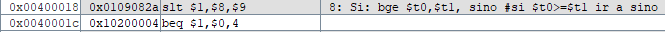
\includegraphics[scale=0.7]{img/proy/bge.PNG}}
    \caption{Conjunto de instrucciones implementadas por MARS para simular el funcionamiento de la pseudoinstrucción \texttt{bge}}
    \label{fig:my_label}
\end{figure}


\subsection*{Cuestión 2.15}
El siguiente código traducido desde el pseudocódigo sería:
\begin{listing}[h]
\begin{minted}[linenos,frame=single]{nasm}
.data
dato1: .word 30
dato2: .word 40
res: .space 1


.text
main: 
lw $t0,dato1($0) # cargar dato1 en t0
lw $t1,dato2($0) # cargar dato2 en t1
and $t2,$t2,$0


blt $t0,$t1, else
sub $t2, $t0, $t1
j skip

else: 
    sub $t2, $t1, $t0
    
skip: 
    sb $t2,res($0) # almacenar $t2 en res

\end{minted}
\end{listing}

\subsection*{Cuestión 2.16}
El pseudocódigo correspondiente al ejemplo sería:

\begin{listing}[h]
\begin{minted}[linenos,frame=single]{nasm}

VARIABLES
ENTERO: dato1=30; dato2=40, dato3=-1; res;
INICIO
Si (dato3 < dato1):
    res = 1
Sino:
    Si (dato3 <= dato2):
        res = 0
FIN
\end{minted}
\end{listing}

\newpage



\subsection*{Cuestión 2.17}
El valor cargado en \texttt{res} en este caso es \texttt{1}, ya que se cumple el primer caso de la cadena de condicionales: \texttt{(-1 $<$ 30)}. En el caso de que \texttt{dato1=40} y \texttt{dato2=30} ocurriría lo mismo, pues se seguiría cumpliendo la primer condición: \texttt{(-1 $<$ 40)}.

\subsection*{Cuestión 2.18}
El siguiente código traducido desde el pseudocódigo sería:
\begin{listing}[h]
\begin{minted}[linenos,frame=single]{nasm}
.data
dato1: .word 40
dato2: .word 30
dato3: .word -1
res: .space 1
.text

main: 
lw $t1,dato1($0) # cargar dato1 en t1
lw $t2,dato2($0) # cargar dato2 en t2
lw $t3,dato3($0) # cargar dato3 en t3

and $t4,$t4,$0

bge $t3,$t1,entonces
j endif
entonces:
        ble $t3,$t2, entonces2
        j endif
entonces2:
        addi $t4,$0,1
endif:
     sb $t4,res($0) # almacenar $t4 en res

\end{minted}
\end{listing}


\section*{Estructura de control repetitiva \textit{while}}

\subsection*{Cuestión 2.19}
El programa que implementa la función del bucle \texttt{while} trabaja de la siguiente manera: primeramente, se carga la cadena en un registro temporal \$t0 y se inicializa el contador de letras en el registro \texttt{\$t2} en \texttt{0}. Luego, empieza la implementación del bucle con la etiqueta \textbf{\texttt{mientras}}, cuya primer instrucción es almacenar en una variable temporal \$t1 el primer caracter de la palabra. Una vez almacenado dicho byte, llega la condición de salida, la cual es cuando ya no quedan palabra por recorrer en memoria y, por coincidente lo que le siguen son espacios de memoria con el valor \texttt{0}. Por lo cual, mientras \$t1 no sea \texttt{0}, el bucle continuará. El bucle continúa sumando los contadores \$t2 (nuestra solución) y \$t0 (logrando así un ``corrimiento'' de caracteres en la palabra). Por último se utiliza la instrucción \texttt{j mientras}, la cual nos devuelve a donde empezó el loop. Una vez se haya conseguido la condición de finalización del bucle, entonces guardamos el contenido de \$t2 en nuestra solución, con el nombre de \texttt{n}.

\subsection*{Cuestión 2.20}
El valor almacenado en \texttt{n} es \texttt{4}, pues el largo de la cadena de caracteres \texttt{``hola''} es \texttt{4}.

\subsection*{Cuestión 2.21}
El siguiente código traducido desde el pseudocódigo sería:
\begin{listing}[h]
\begin{minted}[linenos,frame=single]{nasm}

.data
tira1: .asciiz "hola"
tira2: .asciiz "adios"
.align 2
n: .space 4
.text
main: 
la $t1, tira1 #carga dir. cadena en $t1
la $t2, tira2 #carga dir. cadena en $t2

andi $t0,$t0, 0 #$t0=0

mientras: 
lb $t3,0($t1) #almacenar byte en $t3
lb $t4,0($t2) #almacenar byte en $t4

beq $t3, $0, endloop # (tira1[i])!=0)
beq $t4, $0, endloop # (tira2[i])!=0)
addi $t0,$t0, 1 #$t0=$t0+1
addi $t3,$t3, 1 #$t3=$t3+1
addi $t4,$t4, 1 #$t4=$t4+1
j mientras 

endloop: sw $t0,n($0) #almacenar $t0 en n

\end{minted}
\end{listing}

\subsection*{Cuestión 2.22}
El programa que implementa la función del bucle \texttt{for} trabaja de la siguiente manera: primeramente, se carga el vector de elementos en un registro temporal \$t2, se inicializa el registro \$t3 (el cual contendrá nuestra solución), se inicializa el \$t0 el cual será el ``recorredor'' de nuestro bucle y el cual determinará cuando este debe terminar, junto con \$t1, el cual nos indica el largo del vector. La siguiente línea empieza con la etiqueta \textbf{\texttt{para}}, la cual como su nombre lo indica será la que iniciará el bucle. La primer instrucción del bucle es un salto en rama condicional \texttt{(bgt)}, el cual indica que saltará hacia \texttt{finpara} (el fin del bucle), cuando el registro \texttt{\$t0} (que empieza valiendo \texttt{0}) sea mayor al registro \texttt{\$t1} (el cual indica el largo del vector todo el tiempo). Mientras dicho salto no ocurra, se cargará el primer elemento del vector en otra variable temporal \$t4. Luego, sumaremos a través de la instrucción \texttt{add} el elemento actual (\texttt{\$t4}) a nuestra solución (\texttt{\$t3}), aumentaremos el contador que nos está recorriendo el vector en una unidad, y además desplazaremos el vector en 1 palabra (sumándole 4 a la dirección actual) así el valor de \$t4 se va actualizando en cada vuelta y no recorremos siempre por el mismo elemento. Por último, con el uso de la instrucción \texttt{j}, volvemos a saltar a donde empezó el bucle. Una vez se haya cumplido la condición de salto, entonces guardamos el contenido de \texttt{\$t3} en nuestra solución (\texttt{res}).



\subsection*{Cuestión 2.23}
El resultado almacenado en \texttt{res} es \texttt{41}, que efectivamente es la suma de todos los elementos del vector: (\texttt{$6+7+8+9+10+1 = 41$}).


\subsection*{Cuestión 2.24}
El siguiente código traducido desde el pseudocódigo sería:
\begin{listing}[h]
\begin{minted}[linenos,frame=single]{nasm}

.data
v: .word 6,7,8,9,10,-1,34,23
v2: .space 32
.text
main: 
la $t2,v
la $t3,v2

li $t0,0 #$t0=0
li $t1,7 #$t1=7
para: bgt $t0,$t1,finpara
lw $t4,0($t2) # cargar primer elemento de v
lw $t5,0($t3) # cargar primer elemento de v2

addi $t5, $t4, 1
sw $t5, 0($t3) # guardar contenidos modificados del array

addi $t0, $t0, 1
addi $t2, $t2, 4
addi $t3, $t3, 4

j para #saltar a bucle
finpara: 

\end{minted}
\end{listing}


\end{flushleft}
\end{large}

\end{document}